\documentclass[manuscript]{acmart}
\setcopyright{none}

\bibliographystyle{ACM-Reference-Format}
\usepackage{algorithm}
\usepackage{algorithmicx}
\usepackage{graphicx}
\graphicspath{{figures/}}
\usepackage{float}
\usepackage{array}
\usepackage{booktabs}
\begin{document}
\nocite{*}

\title[AnitoPCG]{Exploring Procedural Content Generation of Saint La Salle Hall in a Customized Game Engine}

\author[1]{Rayo Gabriel Paulo}
\email{gabriel_paulo_rayo@dlsu.edu.ph}
\author[2]{Peñaflorida Carl Joshua}
\email{carl_joshua_d_penaflorida@dlsu.edu.ph}
\author[3]{Arceo Eric Christian}
\email{eric_christian_arceo@dlsu.edu.ph}
\affiliation{%
    \institution{De La Salle University}
    \city{Manila}
    \country{Philippines}
}

\renewcommand{\shortauthors}{Rayo, et al.}

%\address[1]{De La Salle University Laguna Campus, LTI Spine Road, Brgys. Binan and Malamig, Binan, Laguna 4024, Philippines}
%\address[2]{Graphics, Animation, Multimedia, and Entertainment (GAME) Lab - De La Salle University}

\date{February 18, 2026}

\begin{abstract}
Procedural Content Generation (PCG) is the automated content generation technique widely used in game development, urban planning, digital heritage, and educational simulation. It has become an increasingly beneficial tool in three-dimensional asset creation. Very few PCG technologies are built to support domain-specific environments like schools and universities. As such, this project proposes the development of a PCG system specifically for generating De La Salle University Manila (DLSU Manila) buildings, particularly those that are Neo-Classical in architectural style. This will be achieved through the creation of a C++ PCG 3D editor tailored for procedurally generating DLSU buildings and assets designed to replicate real-life structures.
\end{abstract}

\begin{CCSXML}
<ccs2012>
 <concept>
  <concept_id>10010147.10010371.10010387</concept_id>
  <concept_desc>Computing methodologies~Graphics systems and interfaces</concept_desc>
  <concept_significance>500</concept_significance>
 </concept>
</ccs2012>
\end{CCSXML}

\ccsdesc[500]{Computing methodologies~Graphics systems and interfaces}

\keywords{computer graphics, procedural content generation, neoclassical architecture, game engine}

\maketitle

\newpage
\tableofcontents

\newpage
\section{Introduction}

\subsection{Overview of Current Technology}
Procedural Content Generation (PCG) is the automatic generation of content through rules and constraints. It is a feature most commonly used in game development for its efficiency in terms of time consumption and labor. Using algorithms, developers are able to spawn or generate assets procedurally. PCG enables designers to create games with diverse environments and levels, which ultimately results in a more satisfying and immersive experience. It is employed to increase replay value, reduce production cost and effort, to save storage space, or simply as an aesthetic in itself \citep{summerville2017}.

In the context of games, titles like \emph{Minecraft} and \emph{Terraria} demonstrate the use of PCG to generate expansive, varied environments without manual design \citep{shaker2016}. This approach significantly reduces development time and resource demands while increasing replayability and adaptability \citep{lazaridis2024}.

PCG techniques are also being integrated into toolchains and wrappers compatible with 3D modeling and scene management software such as Maya, Blender, Unity, and Unreal Engine, allowing procedural methods to drive content creation pipelines. In architectural modeling and digital twin development, for instance, PCG is used to automate the generation of parametric building facades, road networks, and city layouts, which can then be exported into modeling environments for further refinement or simulation \citep{muller2006, parish2001}.

However, one documented challenge in current PCG applications—particularly in game environments—is the tendency for generated content to appear repetitive or generic, reducing the perceived authenticity of spaces like cities or architectural scenes \citep{togelius2013}.

Addressing this issue is a key area of research, especially in attempts to refine structural detail, variety, and cultural fidelity in procedurally generated models.

Beyond entertainment, PCG is gaining traction in areas such as urban planning, digital heritage, and educational simulation. Urban environments, much like virtual game worlds, require structured layouts and detailed asset placement, making them suitable for automated generation. Studies have shown that PCG can aid in generating realistic 3D cityscapes for planning, analysis, and visualization purposes, thereby supporting more efficient design workflows and enabling scenario testing in virtual simulations \citep{kim2018, parish2001}.

Academic venues such as SIGGRAPH, CASA, and the IEEE Conference on Games regularly publish advancements in PCG methods for urban modeling, cultural heritage reconstruction, and virtual tourism \citep{watson2008}.

For institutions such as universities, PCG offers a scalable way to replicate campuses in digital form, which can be used for educational tools, interactive simulations, and virtual tours. This presents opportunities across disciplines—from computer science and architecture to digital art and cultural studies—to explore generative systems both as research tools and practical applications for content creation. Aside from PCG, there is also already a mature body of software in the field of scene editors (e.g. Unity, Unreal Engine, Blender), most of them are built for general purposes, which involve manual creation of the assets. Very few of them are built to support PCG, specifically for domain-specific environments like schools/universities \citep{smith2011, togelius2016}.

As a solution, professionals have developed plug-ins that users can integrate into modern game engines or their own game engines, which allows the use of PCG techniques. These plug-ins are usually developed using languages like C++ and C\#, and are made as modular components.

\subsection{Statement of the Problem}
Due to the lack of PCG tools tailored for architectural modelling, this project aims to address the limitations of existing procedural content generation tools in accurately replicating neo-classical architecture. It seeks to develop a system that can generate accurate 3D models of DLSU buildings, with a focus on Neo-Classical design elements.

\begin{figure}[H]
    \centering
    
\includegraphics[width=1.0\linewidth]{figures/Slide1.jpg}%
    \caption{Concept diagram of the overview of current technology of PCG}
    \label{fig:overview_pcg}
\end{figure}

\subsection{Project Objectives}
Our main objective is to create a procedural content generation method suited for DLSU buildings. The 3D scene editor that implements this method will be named “Anito Builder.” The specific objectives of this project are as follows:

\begin{enumerate}
    \item Analyze and identify the architectural style of DLSU buildings, with the aim of understanding the underlying design principles and techniques necessary for accurate replication.
    \item Create DLSU-themed building assets which includes both the modeling and texturing of the assets. 
    \item Create an art book, as evidence of the architectural study, that will showcase a selection of neoclassical architecture from both the real life and the game world as well as side-by-side comparison of the references and the recreated DLSU-themed buildings.
    \item Create a PCG method that can generate DLSU Architecture.
    \item Evaluate the created PCG method through a 3D scene editor with a series of qualitative and quantitative tests such as usability tests and quality tests.
\end{enumerate}

\subsection{Scope and Limitations}
The project will focus on procedurally generating aspects of the buildings at De La Salle University. In particular, the project will focus on procedurally generating walls of the Saint La Salle Hall, using neo-classical architecture as a reference, which is a type of architecture from the 18th century that emphasizes symmetry and grandeur. Inspired by the classical architecture of ancient Greece and Rome, it is commonly characterized by simple geometric forms and symmetry. This scope will allow the project to demonstrate its ability to handle repeated patterns, as well as stretched patterns, without looking distorted. 

However, some buildings and structures cannot be generated due to copyright issues or other legal reasons, and the researchers will not be able to get official building schematics, making all generations inspired by Lasallian architecture instead of a one-to-one match of the real-life buildings/locations. This includes murals, sculptures, and artworks that can be found within or on the buildings. Similarly, floor plans, internal designs, and administrative rooms or buildings cannot be obtained or recreated without permission.

As mentioned, the project will revolve around the walls of La Salle Hall. And to be able to develop a PCG method for generating La Salle Hall, it is necessary to create the accompanying pillars, columns, windows, and anything that supports or encloses the wall. The project will not create models for any props like trash cans, food carts, and lamp posts since such objects are not part of a building. Instead, the focus will be on the parts that make up the building.

The models to be used in this project will be made from scratch in Blender, since any engravings or statues will not be covered due to legal concerns. The decision to use Blender is due to the extensive amount of plug-ins available for the program, increasing the speed and efficiency in creating 3D assets. Blender is a free software with precision modeling that is perfect for modeling architectures that require symmetry and proportionality. With the help of modeling features like array, subdivision, and deform modifiers, artists will be able to produce highly-detailed models. Additionally, to develop further understanding of how assets, especially textures, behave when they are used for PCG methods, artists are going to utilize current existing PCG plugins and built-in features for Blender during the modelling process. This will not only help artists create models and textures that better fit the ideal output of the project, but doing so will also help the team determine what kind of PCG method is the most optimal choice. As for the textures, they will be made with the help of Substance Painter and Blender itself. Substance Painter uses Physically-Based Rendering (PBR) which is perfect for simulating real-world lighting conditions. It depicts materials like marble and stone realistically, and since the assets that are going to be created are mostly buildings, the project will greatly benefit from it. Additionally, Blender hosts a powerful shading node system which can be used to create procedural textures that can be used in the project. 3D Open-Source 3D scanning software, such as RealityScan, was considered to speed up the creation of 3D assets; however, due to the nature of the models that will be created, a stylized rendition of the neo-classical architecture, the use of 3D scanning software was omitted from the 3D creation workflow.

The PCG 3D editor will be written in C++. This is because the underlying environment that the project will be tested on is a game engine that is also written in C++. Furthermore, the Vulkan rendering API to be used for the scene renderer is natively in C++. This project will also utilize the CMake build system with the assistance of the VCPKG package manager.

\subsection{Significance of the Study}
Exploring DLSU buildings as a venue for PCG offers significant value. This project can serve as a research on how to structure 3D modelling plug-ins for generalized use in applications. It can provide developers with an idea of how to design their library architecture if they are planning to create a 3D editor. Similarly, it will help 3D artists find a reference in understanding PCG and its application in urban modelling.

Additionally, procedural generation of universities or other similar institutions, specifically DLSU buildings, is rare. PCG-generated buildings and structures can be used as 3D assets for various activities such as advertisements, virtual tours, or simulations that can be showcased to various media.

\section{Review of Related Work}

\subsection{Neo-Classical Architecture}

Neoclassical architecture revives and reinterprets classical Greek and Roman architectural principles, emphasizing symmetry, proportion, and order. Many of the characteristics of Neoclassical architecture focus on symmetry, proportion, order, and monumentality - normally used to express personal identity, civic values or political ideologies. Figure 3 showcases architectures with neoclassical features.

\begin{figure}[H]
    \centering
    
\includegraphics[width=1.0\linewidth]{figures/Slide2.jpg}%
    \caption{Collection of Neo-classical Architecture, Jardin des Tuileries, Pallandiana (Viscenza), Palace of Versailles, Brandenburg Gate, Pantheon (Assassins’ Creed Unity), and the Opéra Garnier}
    \label{fig:overview_pcg}
\end{figure}

Although previous studies and articles have slightly varying definitions for neoclassical architecture, there are similarities that make it easier to understand and determine what makes an architecture neoclassical. As mentioned, neoclassicism is seen as a continuity of ancient Greek and Roman architecture, making its defining characteristics seem familiar. Based on previous studies, Table 1 shows a summary of the characterizing features of neoclassical architecture.

Neoclassical architecture draws inspiration from the forms and ideals of ancient Greece and Rome, not simply for decorative purposes but to reflect a deeper cultural aspiration for order, rationality, and timeless beauty (Watkin, 2005). Central to this architectural movement is the use of classical orders—Doric, Ionic, and Corinthian—which provide a structured and proportioned system that guides the design of columns, entablatures, and facades (Summerson, 1980). These classical foundations support the monumental character often seen in neoclassical buildings, which are typically large in scale to convey a sense of power, permanence, and civic pride. This monumentality and grandeur made the style particularly fitting for government institutions, museums, and universities—spaces meant to embody collective ideals and stability (Bergdoll, 2000; Honour, 1968).

At the same time, neoclassicism is marked by a deliberate simplicity and restraint, distancing itself from the dramatic excesses of the Baroque. It favors clean lines, clear geometry, and measured ornamentation that reflect ideals of clarity and discipline (Watkin, 2005). These qualities align with the Enlightenment's emphasis on rationality and idealism, where structured, well-ordered spaces were thought to mirror and even promote the intellectual and moral progress of society (Summerson, 1980). Finally, the principles of symmetry and proportionality are fundamental to the style, with mathematically precise layouts that evoke harmony and balance. These design decisions were not purely aesthetic—they embodied a philosophical belief in the power of reason and the pursuit of ideal form (Summerson, 1980; Kruft, 1994).

\begin{table}[h!]
\centering
\caption{Summary of the Characterizing Features of Neoclassical Architecture}
\label{tab:neoclassical_features}
\renewcommand{\arraystretch}{1.3} % adds vertical spacing
\begin{tabular}{>{\raggedright\arraybackslash}p{4cm} >{\raggedright\arraybackslash}p{10cm}}
\toprule
\textbf{Feature} & \textbf{Definition} \\
\midrule
Classical Antiquity & Revives the architecture of ancient Greece and Rome (Watkin, 2005). \\
\addlinespace
Classical Orders & Defines the proportion and structure of neoclassical buildings (Summerson, 1980). \\
\addlinespace
Monumentality and Grandeur & Projects a sense of power, permanence, and civic pride (Bergdoll, 2000; Honour, 1968). \\
\addlinespace
Simplicity and Restraint & Distinguishes it from the decorative excesses of the Baroque (Watkin, 2005). \\
\addlinespace
Rationality and Idealism & Embodies the era’s emphasis on rationality and the belief that structured, ordered design could reflect and promote human progress (Summerson, 1980). \\
\addlinespace
Symmetry and Proportionality & Reinforces ideals of balance and harmony through mathematically precise relationships in form and layout (Summerson, 1980; Kruft, 1994). \\
\bottomrule
\end{tabular}
\end{table}

\subsection{De La Salle University Manila Architecture}
Currently, there are 19 buildings within DLSU - Manila, 9 of which are classroom buildings and the rest are administrative and auxiliary buildings (De La Salle University, n.d.). The 9 classroom buildings included are named as the following:

\begin{itemize}
    \item St. La Salle Hall
    \item St. Joseph Hall
    \item Br. Andrew Gonzales Hall
    \item Vleasco hall
    \item Yuchengco Hall
    \item Don Enrique T. Yuchengco Hall
    \item Henry Sy Sr. Hall
    \item Science and Technology REsearch Center
    \item John Gokongwei Sr. Hall
\end{itemize}

\begin{figure}[H]
    \centering
    
\includegraphics[width=1.0\linewidth]{figures/Slide3.jpg}
    \caption{Collection of Neo-classical features of DLSU Manila buildings}
    \label{fig:workflow}
\end{figure}

These buildings can be classified into different architectural styles, mainly due to the time period they were constructed in and the person/organization they were named after. They could be classified as neoclassical architecture, modernist architecture, and even art deco. In relation to the scope of this project, only two DLSU buildings that have clear influences of Neoclassical architecture will be focused on. Using Table 1 as a criteria, we classify La Salle Hall and Yuchengco Hall as having a neoclassical architectural style. Table 2 shows a clear classification of some of the buildings listed above.

\begin{table}[H]
  \centering
  \caption{Classification of Yuchengco Hall and La Salle Hall}
  \label{tab:classification}
  \begin{tabular}{@{}lll@{}}
    \toprule
    Building & Year(s) & Style / Features \\
    \midrule
    St. La Salle Hall & 1920--1924 & Neoclassical: classical orders, symmetry \\
    Yuchengco Hall & 2000--2002 & Neoclassical influences: Corinthian columns \\
    \bottomrule
  \end{tabular}
\end{table}

\subsection{PCG Tools for Artists}
Modern 3-dimensional modelling software (e.g., Blender, Houdini, Maya) offers tools for PCG (Hanif et. al., 2025, SideFX, n.d., Autodesk University, n.d.) These come in the form of plug-ins that other people have created, specific to work within that particular software (Mullane, 2007). However, there is a need for a much more general product that can be used by others for integration into their own applications (i.e., custom game engines). Very few publicly available libraries focus on the ability to procedurally generate meshes. Most publicly available resources focus on aiding the mathematical computations needed for procedural generation (Müller et al., 2006).
	
Unreal Engine 5 is a modern Game engine that has procedurally generated content built into the engine. The software allows users to import their own assets and make PCG landscapes, which have been used by many game developers over the years, however, one common issue with Unreal Engine 5 is the low performance of the engine on many systems. Unreal Engine 5 has many features that are meant to make games visually appealing. Features such as Lumen and Ray Tracing allow developers to make amazing-looking games with very little effort, but because of this, many scenes become hard to optimize, and this extends to the PCG content the engine creates. Many scenes become hard to run, and for the developers, it becomes hard to generate because their systems lack the speed necessary to run all these features.

\section{Concepts}

\subsection{Concepts in Neo-Classical Architecture}
It was mentioned in Table 1 that one of the characteristics of neoclassical architecture is that they follow classical orders. These classical orders are considered to be the foundation of classical architecture. They are systems of architectural design first used in ancient Greece and then expanded by the Romans. Each order is a system and explains the proportions and structures of buildings. Each classical order consists of: (Figure 4 shows a diagram of a classical order).

\subsection{Concepts in Procedural Content Generation}
PCG methods may be categorized into low-human-intervention methods (e.g., noise-based generation) and high-human-intervention methods (e.g., rule-based models such as shape grammars and L-systems).

There is a pedestal that usually serves as the base of the order. However, in some structures, the pedestal is not present. On top of the pedestal is where the column starts. The base is typically what makes up the bottom part of the column except for doric columns as they don’t have a base. Above the base is the shaft which is the longest part of the classical order. They are usually fluted and tapers towards the top (a refinement called entasis). At the very top of the column is the capital which varies in design and structure depending on the type of order. The entablature is what comes on top of the columns and is divided horizontally, like the column. Similar to the capital, Entablatures are different depending on the type of order. However, they all have the same three parts. The architrave that comes on the most bottom, the frieze which comes in the middle and is the most decorative part, and the cornice which tops the entablature. 
Classical orders come in a wide range of styles, appearances, and proportions. These differences arise from their historical origins and symbolisms. There are five different kinds of classical orders: Doric, Ionic, Tuscan, Corinthian, and Composite. (see Figure 5).

\subsubsection{\textbf{Ionic Order}}
Unlike the Tuscan order, the Ionic order is fluted. It has a slender shaft and a height of approximately 8 times its diameter. Its capital has spiral scrolls (volutes) on either side and its entablature has a continuous frieze. It symbolizes femininity, grace, and elegance which supports the use of Ionic columns for the Temple of Athena Nike.

\subsubsection{\textbf{Doric Order}}
The doric order is a unique order in a sense that it does not have a base (see Figure 5). Although there is a base for it shown in the figure above, what is shown is a roman doric order, which has bases unlike greek doric bases that lack it. It has a fluted shaft and is significantly small in terms of proportions. Similar to the Tuscan order, it has a simple echinus and abacus and is meant to symbolize masculinity and strength. Its entablature commonly hosts triglyphs and metopes in the frieze. (Summerson, 1980). They are used for temples and civic buildings such as the Parthenon in Athens.

\subsubsection{\textbf{Tuscan Order}}
As illustrated in Figure 5, the Tuscan order is the simplest Roman order among all of them with an unfluted shaft as well as a simple base and capital. Its entablature is plain and minimally decorated. It lacks the complexity that the other orders have, and instead focuses on evoking a sense of strength and utility. They are commonly used for forts, warehouses, and military buildings.

\subsubsection{\textbf{Corinthian Order}}The Corinthian order is the tallest and thinnest among all the classical orders with its height being 10 times its diameter. Its capital is decorated with acanthus leaves and scrolls; and its entablature is significantly more ornamented than Doric ones, similar to the Ionic order. It symbolizes luxury and beauty and is used for building interiors and monuments dedicated to gods. The most famous example of the Corinthian order is the Pantheon in Rome.

\subsubsection{\textbf{Composite Order}}
Similar to the Corinthian order, the Composite order is one of the orders with the tallest columns with its height being 10 times its diameter. Its capital is a combination of the Ionic and Corinthian styles, in a sense that it has both the volutes of the Ionic order and the acanthus leaves of the Corinthian order. It symbolizes grandeur and authority and is commonly used in arches and monuments. 
Here is a summary of all the similarities and differences between the five different classical orders:

\subsection{Classifying DLSU-Manila Architecture}
To preserve cultural and historic value, it is important to appropriately classify DLSU buildings. Aside from their functional use, the styles of some of these buildings embody the university’s identity and values. In particular, the La Salle Hall as well as the Yuchengco Hall draws significant influence from neoclassical architecture.

Both La Salle Hall and Yuchengco Hall at De La Salle University–Manila reflect Neo-Classical influences, though to different extents and with varying fidelity to classical orders. La Salle Hall exemplifies the Corinthian order, featuring a fluted shaft, an ornate capital with acanthus leaves and scrolls, and a structured entablature with a plain architrave, clean frieze, and dentil-lined cornice. It is crowned by a sculpted triangular pediment, reinforcing its classical and symbolic stature (Figure 11). In contrast, Yuchengco Hall takes a more interpretive approach. While it incorporates similar elements—a fluted shaft, acanthus-adorned capital, and a dentil cornice—its composition is more restrained. The pediment is left bare, and classical references are simplified to suit a modern context (Figure 12). Despite their differences, both buildings share key Neo-Classical traits: symmetry, proportion, and classical motifs. La Salle Hall adheres closely to formal Corinthian principles, while Yuchengco Hall presents a minimalist, contemporary adaptation. Although some of the remaining buildings seem to be of a similar style as the LS Hall and Yuchengco Hall such as the Saint Joseph Hall, the lack of decorative elements and overall neoclassical features does not qualify it as such. It does incorporate neoclassical features such as symmetry and proportionality, but they are not as clear as the design of La Salle Hall. 

\subsection{Concepts in Procedural Content Generation}
All procedural content generation methods involve an underlying formula. These formulas can be categorized based on its required inputs. Carli et. al (2011) categorizes PCG methods based on how much human intervention is needed in providing the inputs for the formulas. 

Low-human-intervention methods primarily encompass techniques such as noise-based generation and diffusion-based models. Noise-based methods are ones that use mathematical formulas such as Perlin or Simplex noise, to create organic, pseudo-random patterns. These methods are particularly effective for generating naturalistic textures, terrains, and distributions of elements, with human input largely confined to defining initial parameters and mapping noise values to desired features. Conversely, diffusion-based models, a prominent class of generative artificial intelligence, operate by progressively refining random noise into coherent data based on patterns learned from vast training datasets. While their initial training demands significant human effort in data curation and model architecture, the generation phase itself requires minimal input.

In contrast, high-human intervention methods are characterized by explicit human design that micro-manages content generation. One category of this is rule-based models. Rule-based models utilize human experience and knowledge to serve as the basis for pattern induction (i.e., rules) (Zhang, 2025). Rule-based models include shape grammars, L-systems, and cellular automata. Shape grammars are formal systems that apply transformative rules to geometric primitives, enabling the iterative generation of complex designs, commonly seen in architectural and urban planning. Lindenmayer Systems (L-Systems), employ recursive rewriting rules to model fractal structures and biological growth, notably used for realistic plant generation. Cellular automata involve grids of cells whose states evolve based on local rules, leading to emergent complexity suitable for simulating natural phenomena or generating abstract patterns.

Another category of high-human intervention methods is algorithmic procedural generation. This is a method wherein content is produced through a fixed, step-by-step process embedded within an algorithm. This approach relies on a pre-determined sequence of operations applied to specific inputs. This methodological choice prioritizes predictability and reliability.

When creating a software architecture, it is important to note that developers prefer to be able to port a software library across multiple applications where it can be loaded as-is. Portability refers to how easy it is to successfully import and use an external library in your project (International Software Testing Qualifications Board, 2014). Portability is directly proportional to a software's ability for co-existence where it can share resources with other independent software.

A software library is a module or component. This means that it should be a minimal piece of software item that should be testable in isolation. It should define the inputs it can receive, the outputs it will generate, and the underlying logic that it houses. The act of testing a library is called unit/component testing. Other developers may want to create projects that can help a library seamlessly communicate with other projects such as an external application. These projects are called wrappers as they "wrap" the underlying library in a format that the receiving project can understand (Babych, M., 2024).

For this project, the language to be used is C++. This is because C++ is one of the lowest level languages out of the current mainstream languages. A low-level language is one that is close to assembly language (i.e., the language that computers can understand natively) (Ayepeku, F. O. n.d.). A low-level language is important in creating libraries because it makes it easier for higher-level languages to create high-performance wrappers.

When creating libraries in C++, the choice of build system is important. A C++ build system is a tool to assist developers in automating the application's build process. C++ build systems may handle the linking of different libraries together. They may also be responsible for communicating with your package manager, which in turn, makes them responsible for handling dependencies. Linking in C++ means associating a symbol with its definition. One library may have a definition for the symbol, "Vector3." As such, when a developer links this library to their executable, they will now be able to use the Vector3 symbol in their code.

CMake is an example of a build system. CMake is cross-platform, and mainstream across many C++ projects. This in turn, makes it well documented and flexible. CMake uses CMakeLists.txt files to determine how linking between libraries is done.

The application programming interface (API), is the way that programmers will be able to use the library. For object-oriented languages, the API should be anchored on SOLID design principles which include: 

\begin{itemize}
    \item Single Responsibility Principle
    \item Open/Closed Principle
    \item Liskov Substitution Principle
    \item Interface Segregation Principle
    \item Dependency Inversion Principle
\end{itemize}

\section{Methodology}
The artists will be assigned to create the assets to be used by the Anito Builder. This would be imported to the PCG Library's local database, while subsequently being used for the creation of the Art Bible as well. The developers of the PCG Library will handle the creation of the internal logic, and also the subsequent Anito Builder 3D Scene Editor. It is this scene editor that all evaluations will take place.

\subsection{3D Asset Development Workflow}
The development of modern 3D assets has followed a similar process for quite some time now, which is to help make the 3D development process more efficient and to reduce the number of steps needed in creating various assets. The step-by-step process may vary slightly depending on the specific steps needed in creating 3D assets to better match the project, but for PCG content, a workflow process has been generalized into the following steps (Fig., 15). 3D Asset workflows begin with a creative direction, artists and software developers discuss what art style the assets should follow, followed by gathering references, making the mesh models, and then texturing the 3D assets. The chosen workflow has the following steps:

\begin{enumerate}
    \item Stylization and reference gathering: This step is about the stylization of the buildings chosen to be modeled; references and discussions are made here to ensure a consistent art style.
    \item Low-poly mesh modeling: Creating a low poly mesh model will be the start in creating the 3D assets to ensure that all models are easily exportable and workable. This step includes the standardization of the unit of measurement for all models, ensuring that all models follow a specific scale.  In addition to low poly mesh optimization, areas with more detail that require high poly mesh modelling will be created during this step, making them separate models.
    \item Mesh optimization: Once a low poly mesh is created, optimizations and final passes must be done to ensure that all the models are functional and will run well on any program and machine. 
    \item Texturing: Once the mesh of the 3D asset is done, the mesh must be textured. This step includes making normal maps, creating UV maps, and painting the textures for each of the models. In this phase of the 3D asset creation, textures must also be tested to see if lighting effects such as bloom and light reflections work well with the created textures.
    \item Asset integration: The final step is to compile all the 3D assets, ready to be integrated into the PCG Pipeline, allowing the program to use all the created 3D assets (see Figure 16).
\end{enumerate}

To ensure the quality of the generated content, limit creation will be implemented to guide the outputs of the procedural generation system. This involves setting clear constraints—such as size, proportions, and architectural elements—to make sure that the generated buildings are both visually coherent and structurally sound. By doing so, the team can avoid unrealistic results and maintain a consistent design language across all models, ultimately improving the overall quality and usability of the generated content.

\begin{figure}[H]
    \centering
    
\includegraphics[width=1.0\linewidth]{figures/Collection of Modular Assets.png}
    \caption{Flowchart showing the 3D Asset Development Workflow}
    \label{fig:workflow}
\end{figure}

\subsection{Creation of an Art Book}

The 3D models that will be used in the project will be made using real-world and in-game references, including mainly architectural photographs and illustrations. The neoclassical-influenced buildings, specifically, are going to be made following the system of classical orders. As such, it is important to study and learn how they are meant to be constructed and their use to ensure architectural accuracy.

As a product of this, the project includes the creation of an art book that showcases neoclassical architecture both in the real world and in games. It will serve both as a reference material for the group and as a visual and conceptual companion to the models. Through this, the art book aims to illustrate the influence of neoclassical and other historic architectural styles on the current standing buildings of De La Salle Manila.

\subsection{Creation of the Anito builder 3D Editor}

An application named "Anito Builder" will be created. It will be a standalone 3D editor application that aims to allow users to intuitively use the created PCG method to generate custom scenes.

The application will be developed using several libraries. Major libraries to be used include the following (see Table 3):

\begin{table}[h!]
\centering
\caption{Summary of Libraries and APIs Used in the Project}
\begin{tabular}{|p{3cm}|p{10cm}|}
\hline
\textbf{Library/API} & \textbf{Description} \\
\hline
Vulkan & This is the rendering API to be used for the project. Vulkan is used because procedurally generated scenes require heavy optimization. This heavy optimization is something that Vulkan can offer since it lets developers interact with low-level functionality. \\
\hline
SDL2 & This is the window and event management library that will be used. This is because SDL2 already contains most features that are needed for a full-fledged application window. Furthermore, SDL events are preferred over how other window libraries scan for events. \\
\hline
Assimp & The 3D asset importer to be used. Assimp is preferred because it can handle the loading of large models relatively easily — a requirement to be able to use the high-poly modules created. \\
\hline
ImGui & The graphical user interface library to be used for window layout and various types of user interaction. ImGui allows for customizable UI layouts and easier implementation. \\
\hline
\end{tabular}
\end{table}

The main concept of the 3D editor is based on editable blocks similar to what one can find on Unity's Probuilder or Blender's face edit mode. Anito Builder will spawn cubes in which all 4 faces of the cube are selectable and movable in the x-plane, while the cube's height can be controlled by the given inspector.

The cube can be extended by selecting a face and pressing "append" on the editor. By doing so, another cube will spawn with that selected face as a shared face between the old cube and the new cube. This can be done indefinitely to create various building shapes.

This form of shape manipulation is preferred over edge selection, which was the originally proposed plan for an older iteration of Anito Builder. This is because face selection made it more intuitive that neoclassical buildings should follow a layout that is blocky by nature.
After finalizing a block, the user of the application can click a button to turn the block into a procedurally generated version of the Saint La Salle Hall (the block is now not visible at this state).

\subsubsection{\textbf{PCG Library Algorithm}}

The procedural generation of the building is based on the wall subdivisions that are created during the edit phase (wherein the block is still visible). For each subdivision, the PCG method will choose which segment type is used based on various parameters. For instance, the most basic parameters that the PCG method uses is the floor number. For the basic wall, it uses the basic 1st floor model if it is floor number 1. While it uses the basic 2nd+ floor model if it is anything above the first floor.

The PCG library will rely on a simple algorithm which will dictate its construction. The ratios and positioning of each element of the final output is to be specified in the GenerationParams class.

\begin{verbatim}
FUNCTION GENERATE_STRUCTURE(params)

    DECLARE res AS GenerationResult
    SET res.meshes TO EMPTY_LIST

    PROCEDURE ADD_MESH(type, position, scale)
        APPEND new Mesh {
            .type = type,
            .position = position,
            .scale = scale,
            .rotation = Quaternion::Euler(Vector3(0,0,0))
        } TO res.meshes
    END PROCEDURE

    // STEP 1: CALCULATE VECTORS
    DECLARE delta AS Vector3 = params.to - params.from
    DECLARE stepdir AS Vector3 = delta.Normalize()
    DECLARE forward AS Vector3 = stepdir.Cross(params.up).Normalize()
    DECLARE abdistance AS FLOAT = delta.Magnitude()
    DECLARE halfheight AS FLOAT = params.height * 0.5f

    // STEP 2: EXECUTE MAIN WALL SEGMENT LOOP
    FOR x FROM 0 TO abdistance STEP params.pillarInterval

        // Common base position for current segment
        DECLARE segment_center_x AS FLOAT = x + (params.pillarInterval * 0.5f)
        DECLARE base_segment_pos AS Vector3 = params.from + (stepdir * segment_center_x)

        // STEP 2.1: PILLAR PLACEMENT
        DECLARE pillarpos AS Vector3 = params.from + (stepdir * x) + (params.up * halfheight)
        DECLARE pillarscale AS Vector3 = Vector3(0.5f) * params.pillarThickness
        SET pillarscale.y TO halfheight
        CALL ADD_MESH("pillar", pillarpos, pillarscale)

        // STEP 2.2: WALL SEGMENT PLACEMENT
        DECLARE wallpos AS Vector3 = base_segment_pos + (params.up * halfheight)
        DECLARE wallscale AS Vector3
        SET wallscale.x TO params.pillarInterval * 0.5f
        SET wallscale.y TO halfheight
        SET wallscale.z TO params.wallThickness * 0.5f)
        CALL ADD_MESH("wall", wallpos, wallscale)

        // STEP 2.3: ROOF PLACEMENT
        DECLARE roofpos AS Vector3 = base_segment_pos
        DECLARE roofpos_y AS float
        SET roofpos_y TO (params.height + (params.roofHeight * 0.5f))
        ADD params.up * roofpos_y TO roofpos
        DECLARE roofscale AS Vector3
        SET roofscale.x TO params.pillarInterval * 0.5f
        SET roofscale.y TO params.roofHeight * 0.5f
        SET roofscale.z TO params.roofThickness * 0.5f
        CALL ADD_MESH("roof", roofpos, roofscale)
    END FOR

    RETURN res

END FUNCTION
\end{verbatim}

Given a set of inputs, the algorithm will generate a list of objects containing the mesh type and its transformation. This list can be used by the external environment to render the result. The algorithm is a simple loop that iterates over a plane that is defined by the input parameters. Columns and beams will be evenly spaced out across this plane, and a roof will be used to cap each segment of wall.

\subsubsection{\textbf{Using the PCG library in the 3D editor}}

To create the Anito Builder 3D editor, it will utilize the created PCG library's cross-platform C++ API. The 3D editor will take responsibility for loading and caching the meshes that will be used in the procedural generation. The primary output of the PCG library will be an XML that can be read by the 3D editor in order to construct the resulting model inside the scene editor. The following algorithm explains how a developer should use the API in any external project.

\begin{verbatim}
// CALL THE BUILDER
DECLARE params AS GenerationParams FROM ext::AnitoBuilder
CALL ext::AnitoBuilder::AnitoBuilder::Generate WITH params RETURNING builder_result

// READ THE RESULT AND USE EXTERNALLY-LOADED MESHES
FOR EACH objdata IN builder_result.meshes
    CALL create_mesh WITH objdata.position, objdata.scale, Quaternion::Euler(Vector3(0, 0, 0))
END FOR
\end{verbatim}

\subsubsection{\textbf{Viewing and interacting with the result in the 3D editor}}

The 3D editor will be complete with basic camera controls, object selection/movement, inspecting, and saving/serializing. These features will be utilized by users to create and explore the capabilities of Anito Builder.

The 3D editor will have the ability to create an exported .obj file for use in other applications. This is helpful if the user wants to evaluate the output of Anito Builder in an environment they are already familiar with. The 3D editor will also feature a real-time scalable wall user-interface. Where a user can select a pillar, move it, and then the entire wall will be regenerated according to the new specifications and positions.

\subsection{Evaluation}

There will be two parts to the evaluation of Anito Builder: the evaluation of the usability of the 3D editor and the quality of its output.

\subsubsection{\textbf{Evaluation of Anito Builder's usability}}

To evaluate the usability of the Anito Builder 3D editor, participants will be gathered from the student population of De La Salle University Manila. They will be exposed to the 3D editor and be requested to spend both unstructured and structured time in the application.

For the unstructured time, they will just be requested to create and explore the features of the editor without assistance. While for the structured time, they will be asked to complete tasks wherein minimal assistance can be given. The data that will be gathered from these tests are based on the data collected by Kamińska(2022). These include but are not limited to:

\begin{enumerate}
    \item Time to complete tasks
    \item user interactions
    \item Direct observation of the user
    \item Post-experiment interviews
    \item Questionnaires
\end{enumerate}

\subsubsection{\textbf{Evaluation of Anito Builder's output}}

Similarly, the evaluation of the project’s output will come from students based in DLSU Manila. As DLSU Manila students are more familiar with La Salle Hall, it is only appropriate that participants are chosen from their population. The evaluation for Anito Builder’s output will only include the final scene which makes the need for asset development/programming knowledge unnecessary. 

After the participants are able to create scenes, they will be given ample time to examine and explore the scene they have created. This scene will then serve as the basis for their evaluation. They will be asked to answer a survey form adapted from instruments used by previous HCI studies such as Lavie and Taractinsky’s (2004) aesthetics model, Hassenzahl’s pragmatic and hedonic quality dimensions, and the Visual Aesthetic Perception (VAP) scale. On a scale of 1-5, the participants will evaluate the scene based on this criteria: 

\begin{enumerate}
    \item Perceived Architectural Authenticity – measures how well the scene represents known DLSU architecture and its defining features (e.g., columns, facades, building symmetry).
    \item Stylistic Coherence – assesses whether visual elements appear consistent and aligned with a singular architectural style.
    \item Modular Variation and Design Flexibility – captures the user’s perception of how varied yet coherent the generated components are.
    \item Visual Appeal and Layout Clarity – evaluates subjective judgments of aesthetic quality, layout clarity, and overall pleasantness.
    \item Structural Believability – captures whether the forms look physically plausible and grounded in real-world architectural logic.
\end{enumerate}

To complement this perception-based evaluation of the generated scenes, we will also conduct a System Usability Scale (SUS) test to assess the usability of the PCG-based 3D scene editor itself. The SUS is a widely adopted and validated tool in HCI research for quickly gauging overall system usability, and it provides a standardized score that can indicate whether the interface is efficient, intuitive, and accessible to users. This dual-evaluation strategy ensures that the study captures both the user’s visual and architectural impressions of the generated content and the functional usability of the editor that produces it.

Responses to the survey will serve as a means to provide insight into how effective the PCG system captures the look and feel of DLSU Manila. By making the evaluation focus solely on the output and not on the technical aspect of the development, it prioritizes user experience and visual quality. This is to make sure that the generated scenes meet the expectations of the participants in terms of architectural accuracy and design quality without needing any technical background. 

\section{Results}

\subsection{\textbf{Modular 3D Models}}

The 3D models created were made with these standard measurements: x = 1.2m, z = 1.86m, and y dimensions varying with different types of wall segments. While the standard y dimension is 1.56m, in order to replicate the overall structure of the LS Hall accurately, it was necessary to model the different kinds of wall segments it has. This led to certain segments having higher y dimensions. 

\begin{table}[H]
  \centering
  \caption{Standard Measurements of the 3D Modular Wall Segments}
  \label{tab:classification}
  \begin{tabular}{@{}lll@{}}
    \toprule
    Dimension & Size \\
    \midrule
    x & 1.2 \\
    z & 1.86 \\
    y & varies \\
    \bottomrule
  \end{tabular}
\end{table}

The final collection of models can be classified into 7 categories:

    \subsubsection{\textbf{1st Floor Wall Segments}}
    
    Wall segments that can only be used for the 1st floor of the building, as to keep consistency with the real-world counterpart. This includes the regular 1st floor wall segment and the corner version of it that does not have the wall behind it.

\begin{figure}[H]
    \centering
    
\includegraphics[width=1.0\linewidth]{Figures/1st Floor Wall Segments.png}%
    \caption{Render of the textured 1st Floor Wall Segments}
    \label{fig:overview_pcg}
\end{figure}
    
    \subsubsection{\textbf{2nd Floor Wall Segments}}
    
    Wall segments that can only be used for the 2nd floor of the building, as to keep consistency with the real-world counterpart. This includes the regular 2nd floor wall segment and the corner version of it that does not have the wall behind it.

\begin{figure}[H]
    \centering
    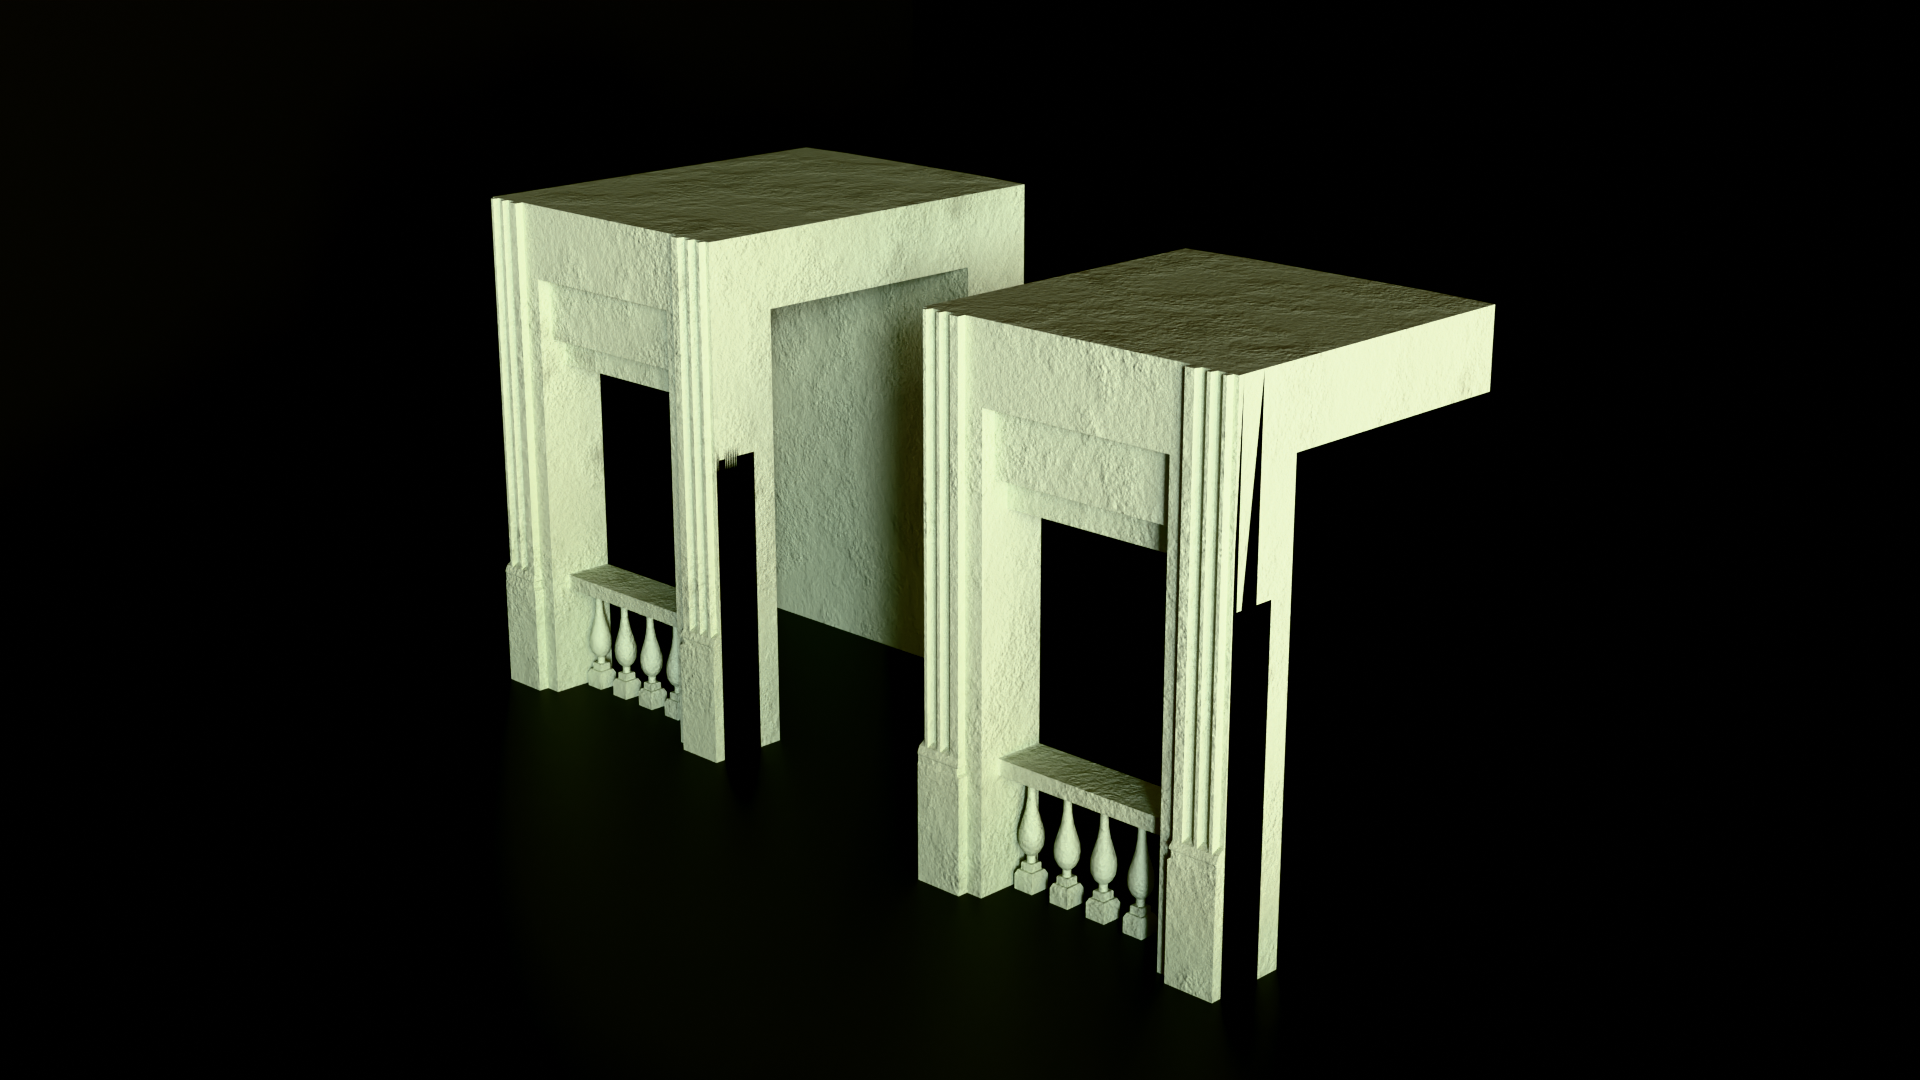
\includegraphics[width=1.0\linewidth]{2nd Floor Wall Segments.png}%
    \caption{Render of the textured 2nd Floor Wall Segments}
    \label{fig:overview_pcg}
\end{figure}
    
    \subsubsection{\textbf{3rd Floor Wall Segments}}
    
    Wall segments that can only be used for the 3rd floor of the building, as to keep consistency with the real-world counterpart. This includes the regular 3rd floor wall segment and the corner version of it that does not have the wall behind it.

\begin{figure}[H]
    \centering
    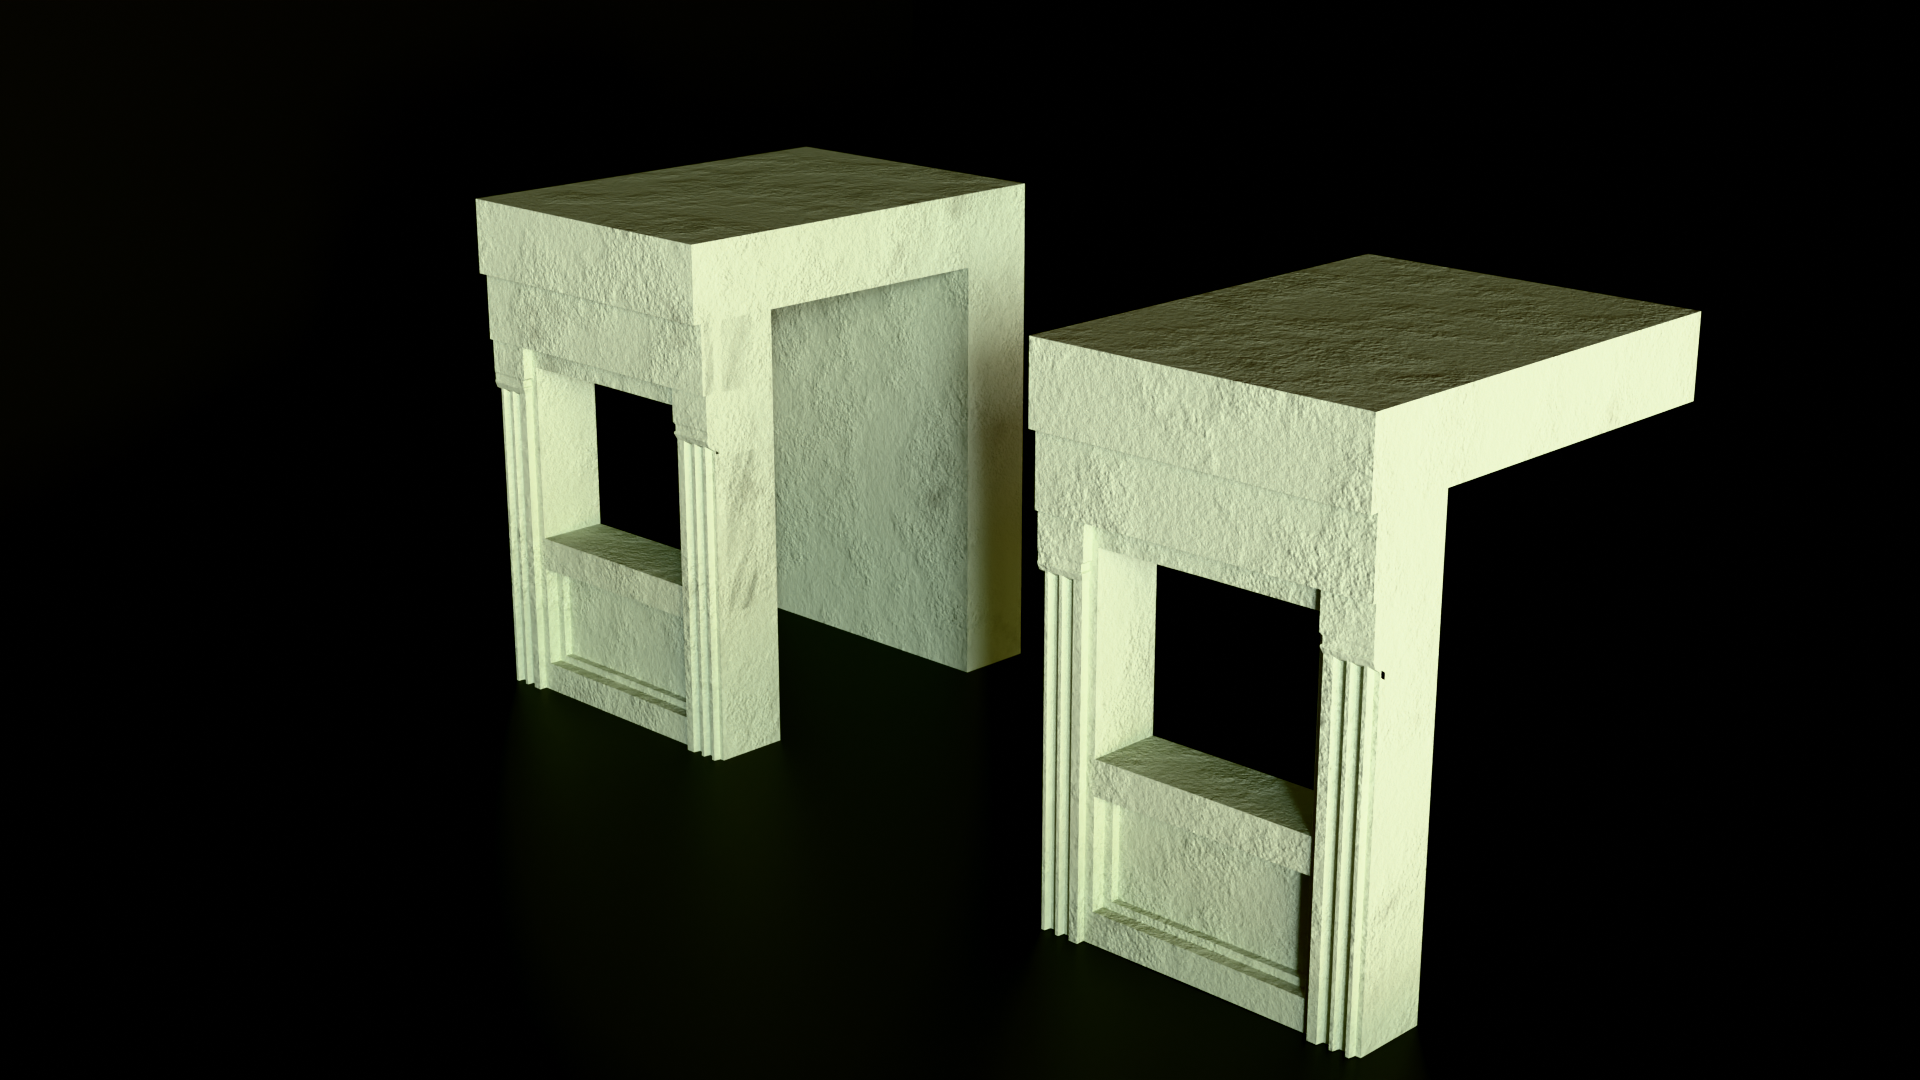
\includegraphics[width=1.0\linewidth]{3rd Floor Wall Segments.png}%
    \caption{Render of the textured 3rd Floor Wall Segments}
    \label{fig:overview_pcg}
\end{figure}
    
    \subsubsection{\textbf{Rooftop Wall Segments}}
    
    Wall segments that can only be used for the rooftop floor of the building, as to keep consistency with the real-world counterpart. This includes the regular rooftop floor wall segment and the corner version of it that does not have the wall behind it.

\begin{figure}[H]
    \centering
    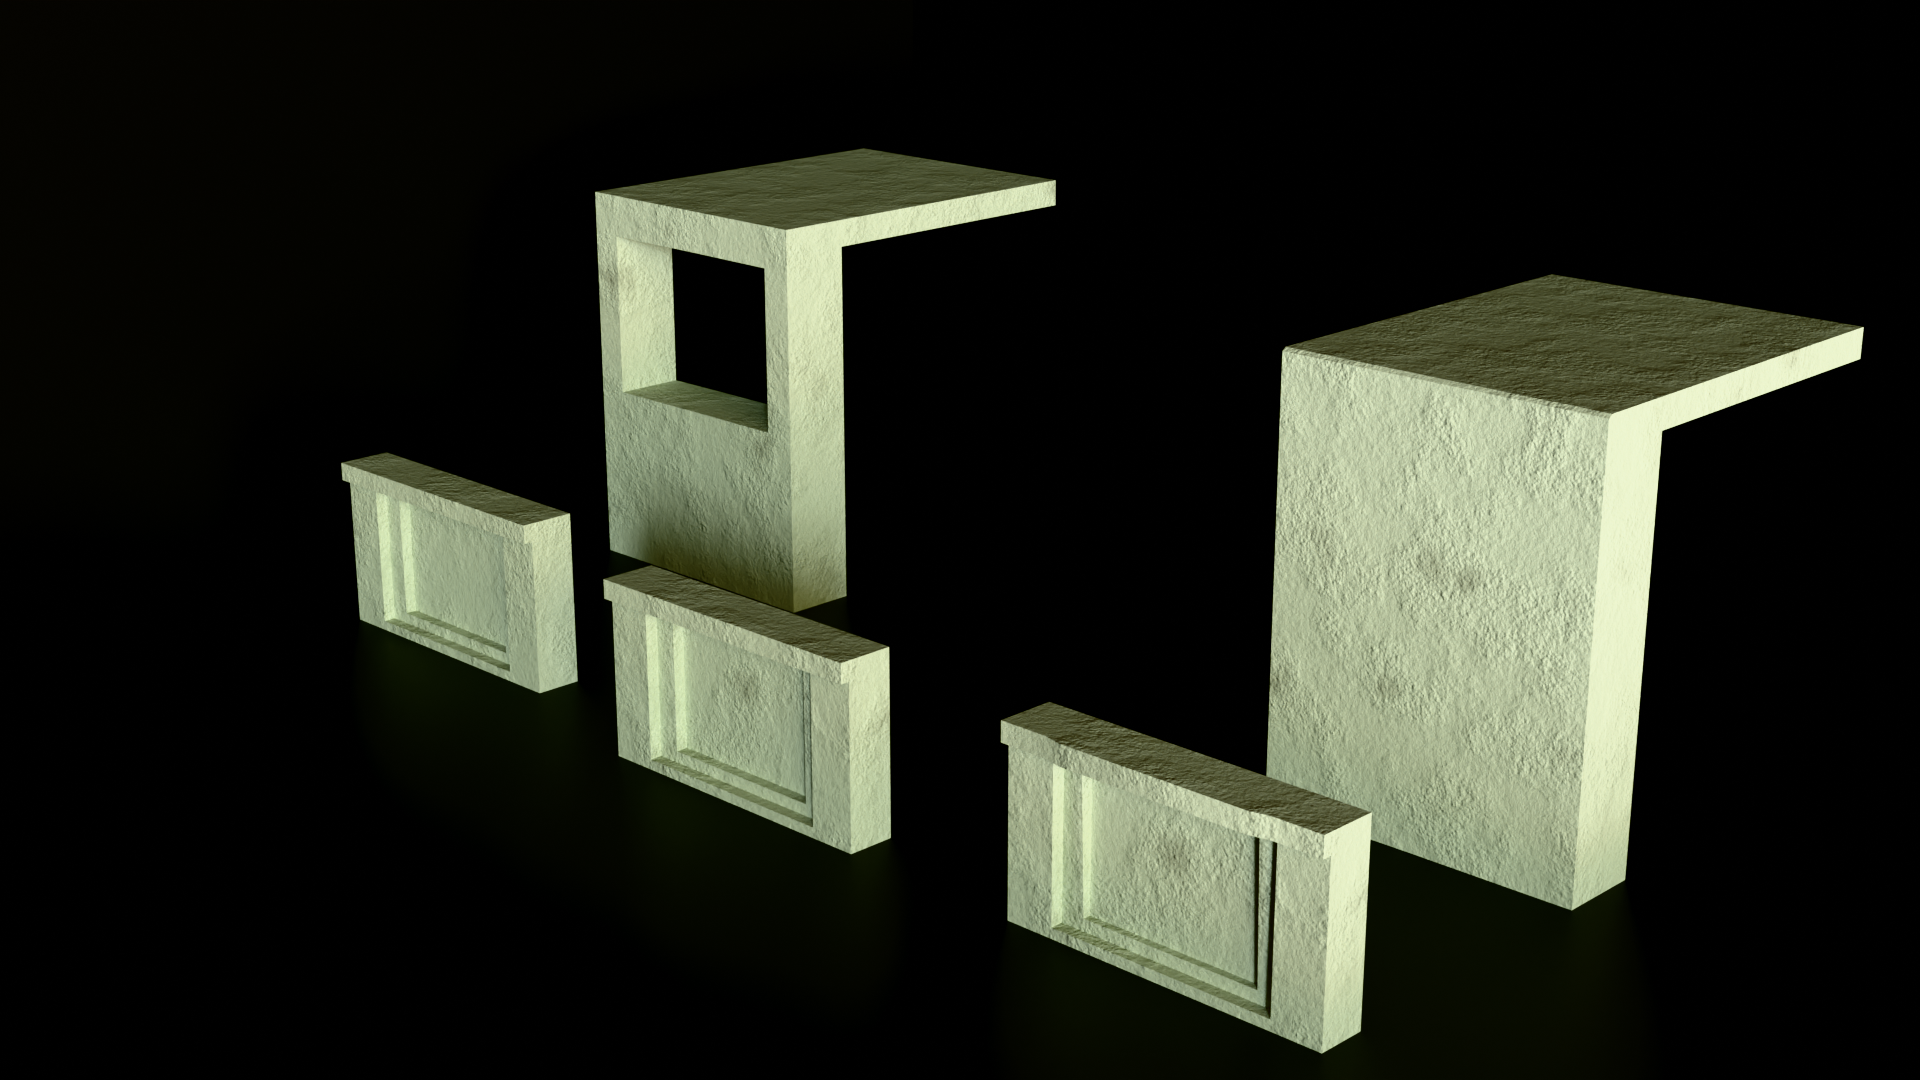
\includegraphics[width=1.0\linewidth]{RooftopFloor Wall Segments.png}%
    \caption{Render of the textured Rooftop Floor Wall Segments}
    \label{fig:overview_pcg}
\end{figure}
    
    \subsubsection{\textbf{2-Segment Wall Segments}}
    
    Wall segments that are a set of 2 wall segments that cannot be used without the other. They were initially made to have a measurement equivalent to a 1x2 or 2x2 of the regular wall segments, but was divided into 2 or 4 regular wall segments for efficiency in terms of exporting to the game engine. These wall segments do not have corner versions and are not meant to be placed in corners.
    
\begin{figure}[H]
    \centering
    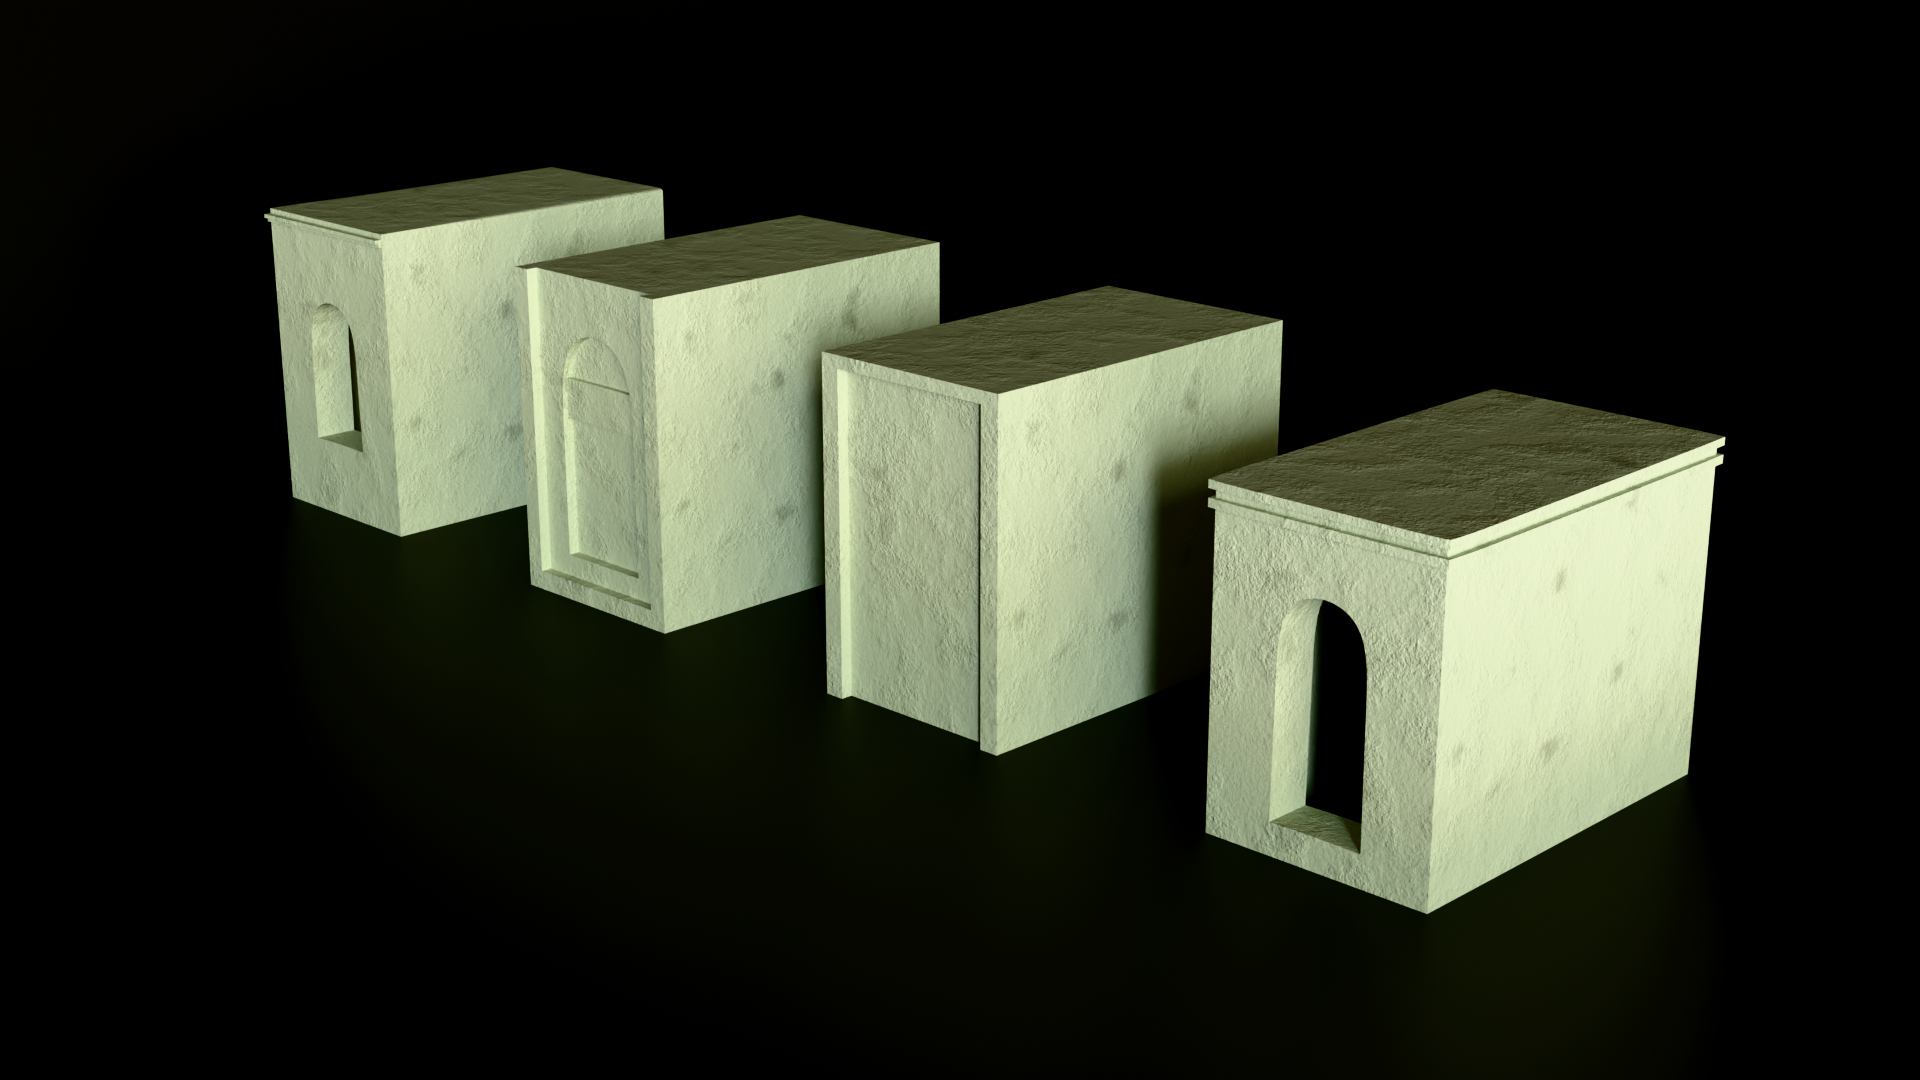
\includegraphics[width=1.0\linewidth]{Wall Segments.png}%
    \caption{Render of the textured 2-Segment Wall Segments Variation 1}
    \label{fig:overview_pcg}
\end{figure}

\begin{figure}[H]
    \centering
    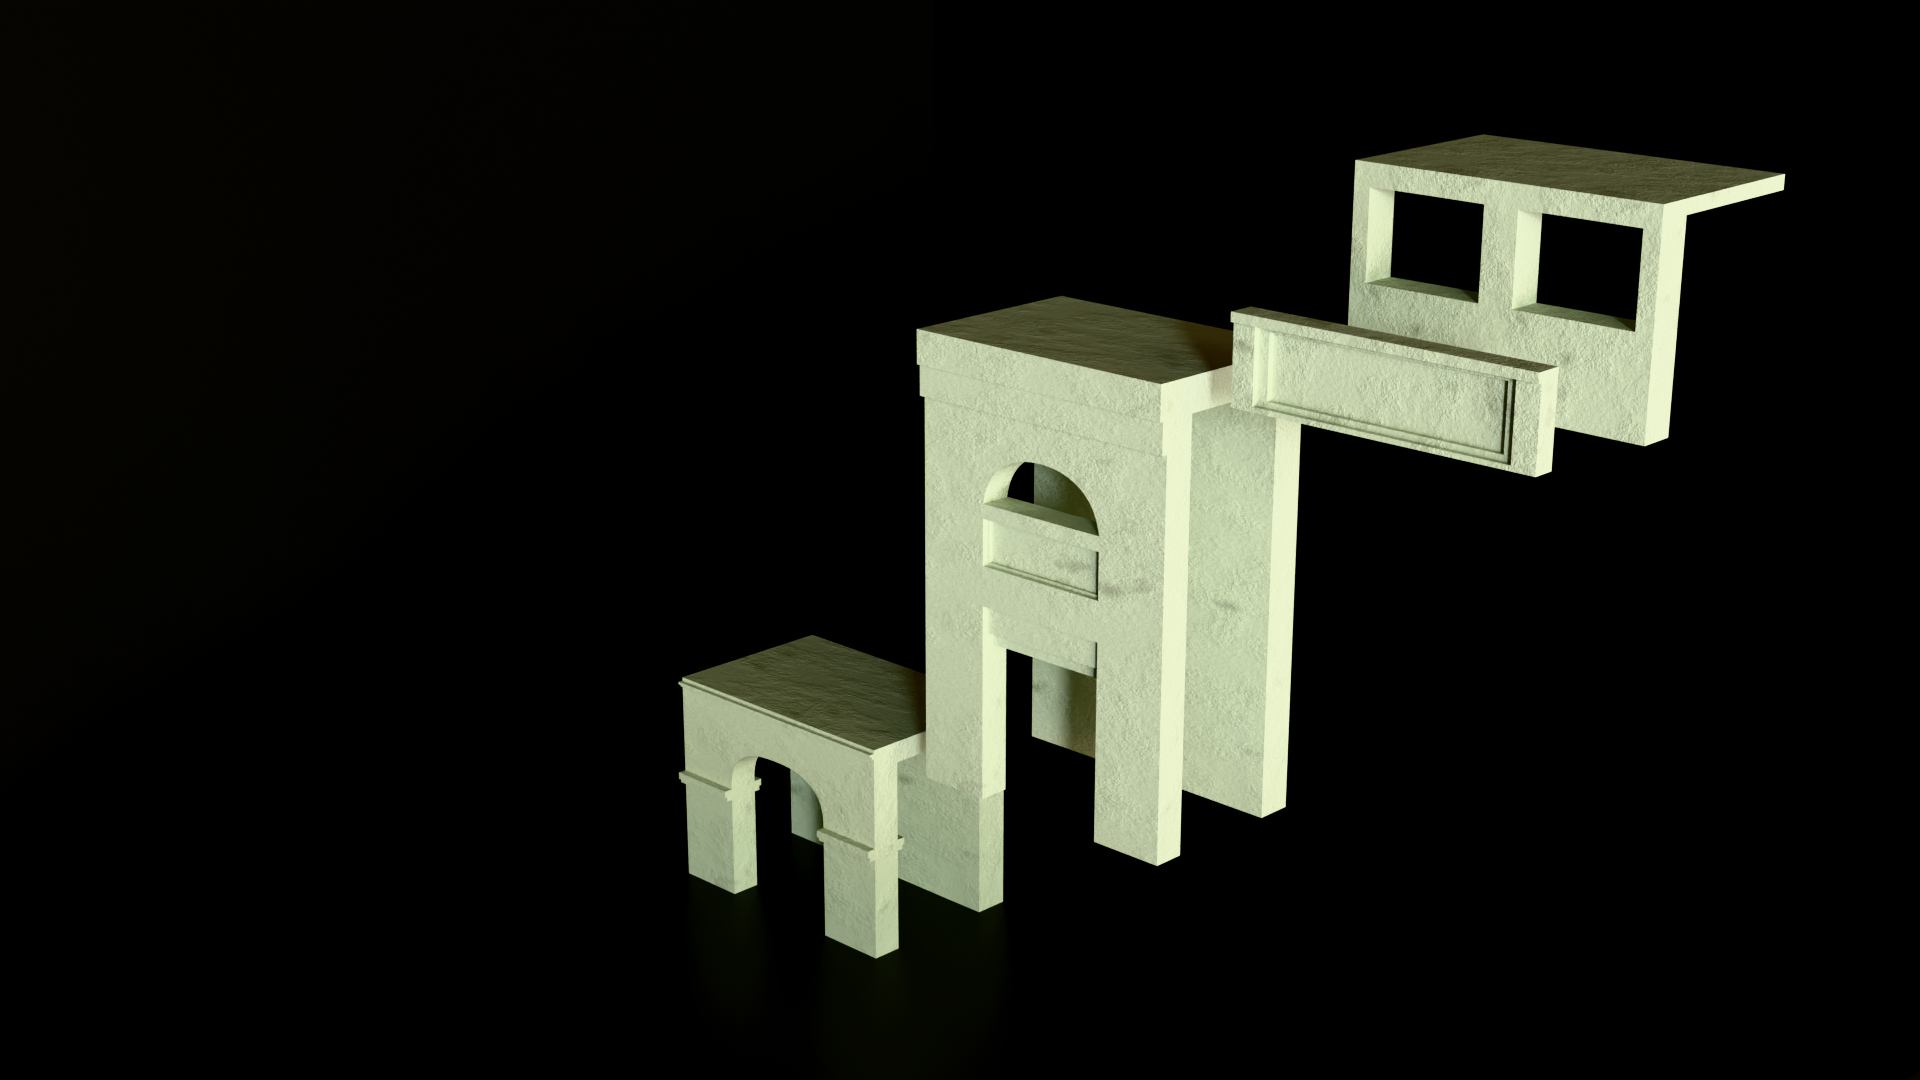
\includegraphics[width=1.0\linewidth]{2-Segment Wall Segments Var 2.png}%
    \caption{Render of the textured 2-Segment Wall Segments Variation 2}
    \label{fig:overview_pcg}
\end{figure}
    
    \subsubsection{\textbf{3-Segment Wall Segments}}
    
    Wall segments that are a set of 3 wall segments that cannot be used without the other. They were initially made to have a measurement equivalent to a 1x3 or 2x3 of the regular wall segments, but was divided into 3 or 6 regular wall segments for efficiency in terms of exporting to the game engine. These wall segments do not have corner versions and are not meant to be placed in corners.

\begin{figure}[H]
    \centering
    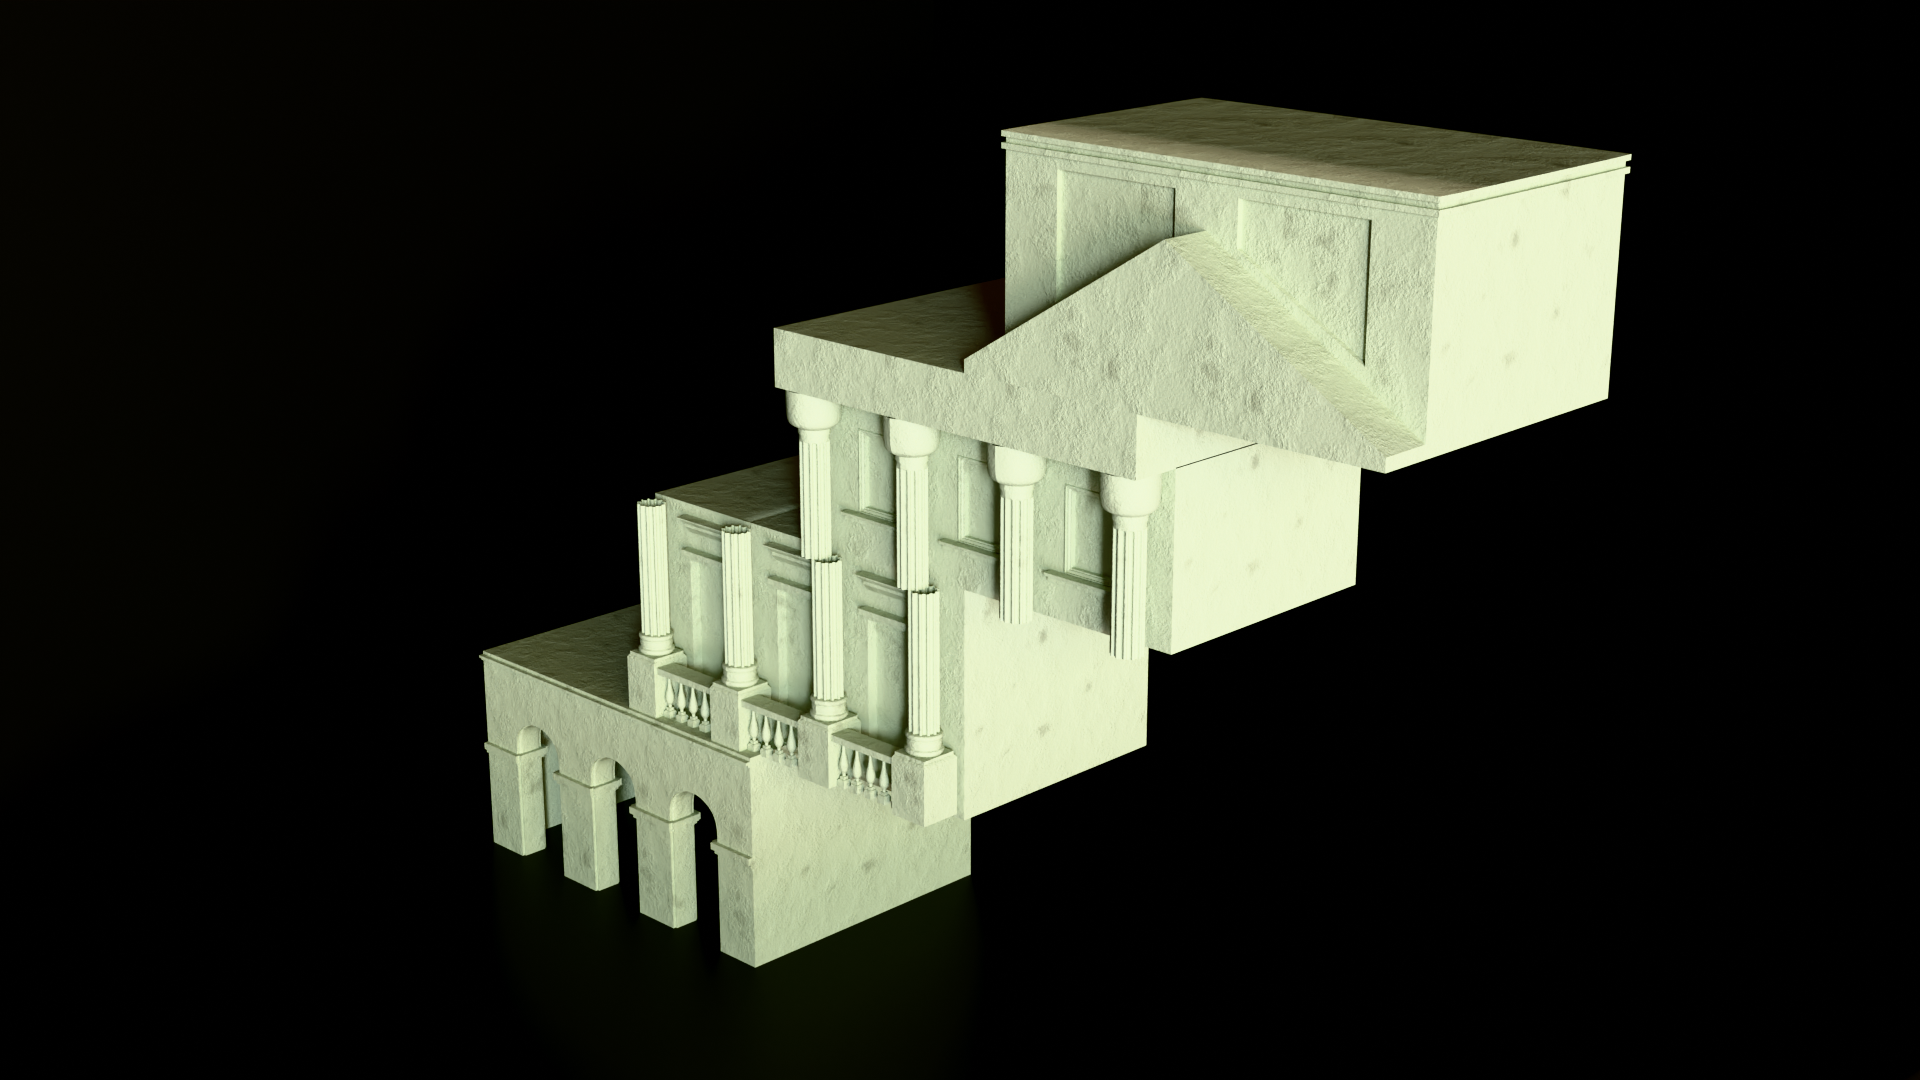
\includegraphics[width=1.0\linewidth]{3-Segment Wall Segments.png}%
    \caption{Render of the textured 3-Segment Wall Segments}
    \label{fig:overview_pcg}
\end{figure}
    
    \subsubsection{\textbf{Wall Segments}}
    
    Wall segments that originally belonged to the center section of the real-world counterpart. These walls can be placed on any floors except for corners.

\begin{figure}[H]
    \centering
    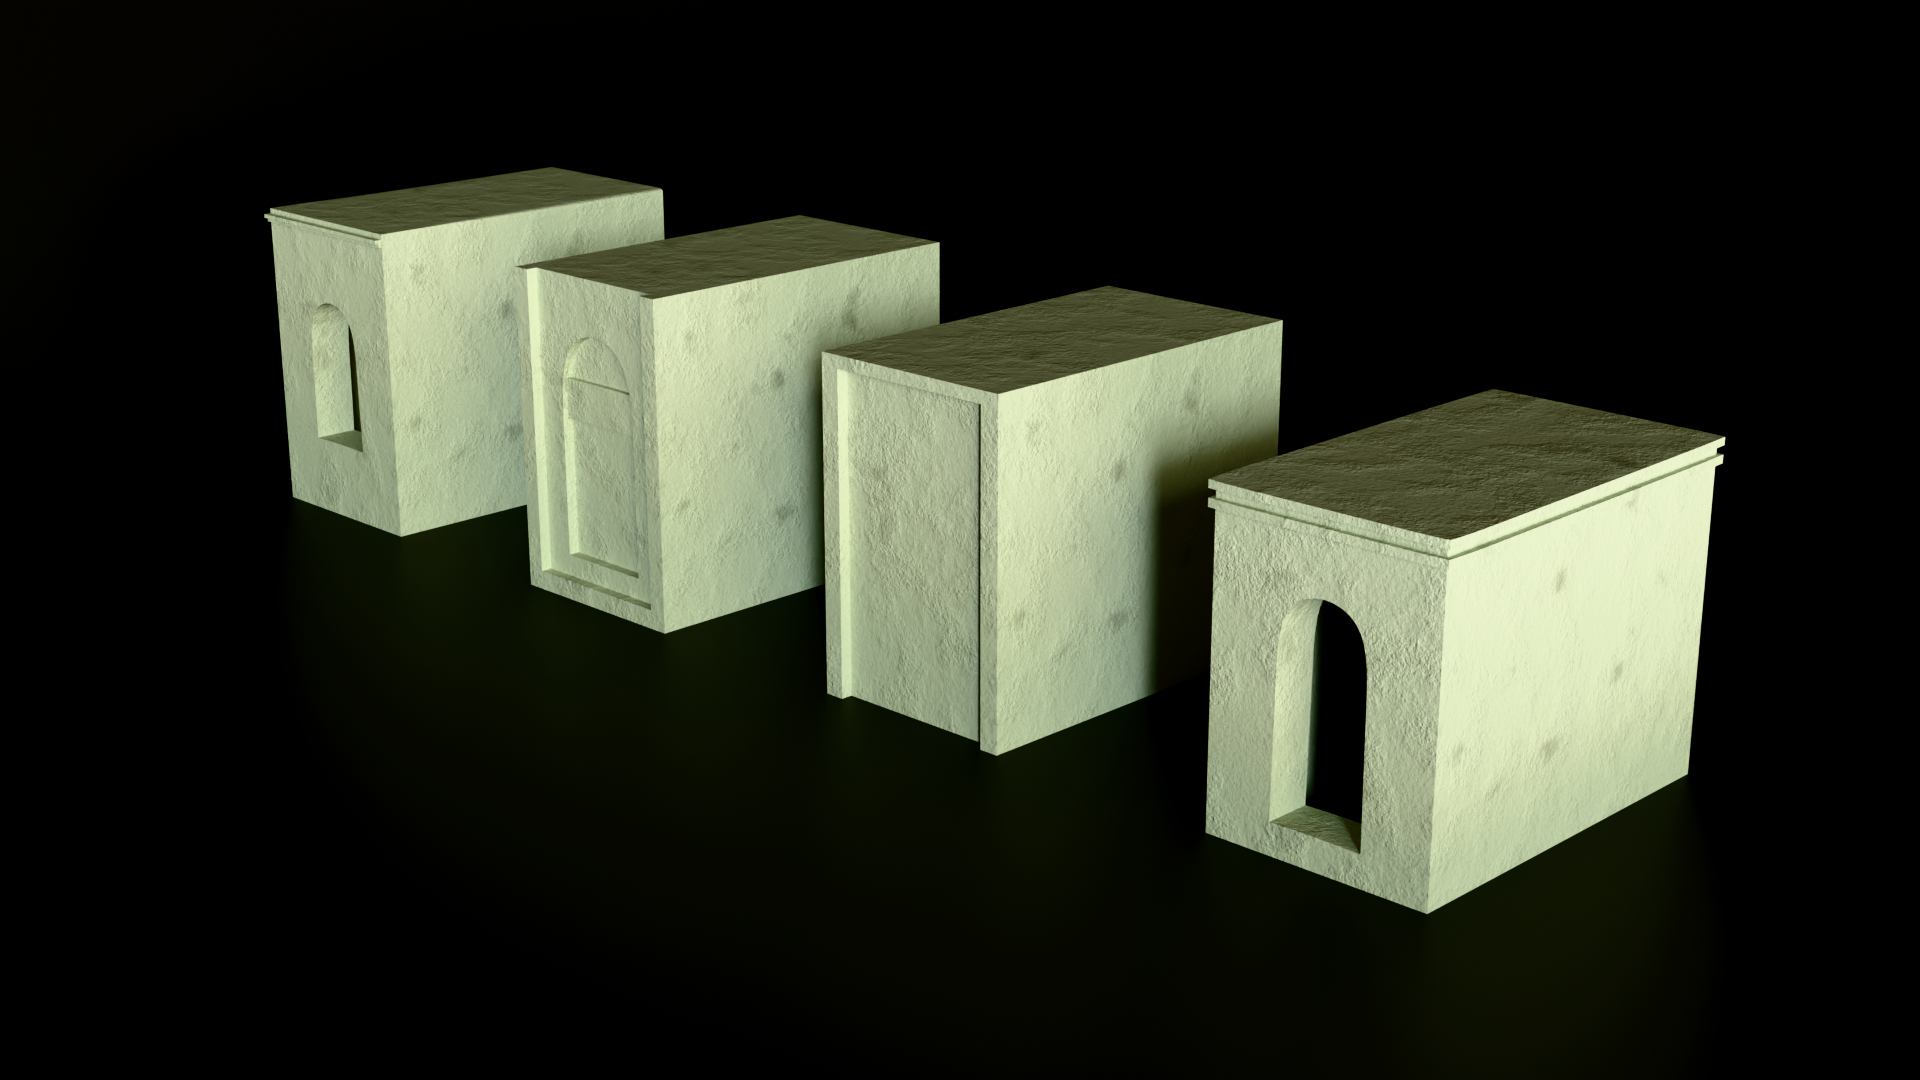
\includegraphics[width=1.0\linewidth]{Wall Segments.png}%
    \caption{Render of the textured Wall Segments}
    \label{fig:overview_pcg}
\end{figure}

As a test to determine the models' accuracy and usability, an attempt to recreate the LS Hall building was made. In terms of individual model accuracy, the models have much to improve. The topology of certain models are a bit off from their real-world counterparts. The measurements of the models when compared to the real building seem a little different. This is due to the standardization of measurements to make the models modular and easier to work with. Additionally, the texture of the models lack variety. While the seams might not be obvious, it is not as seamless as expected and a pattern can be observed when the models are lined up. 

\begin{figure}[H]
    \centering
    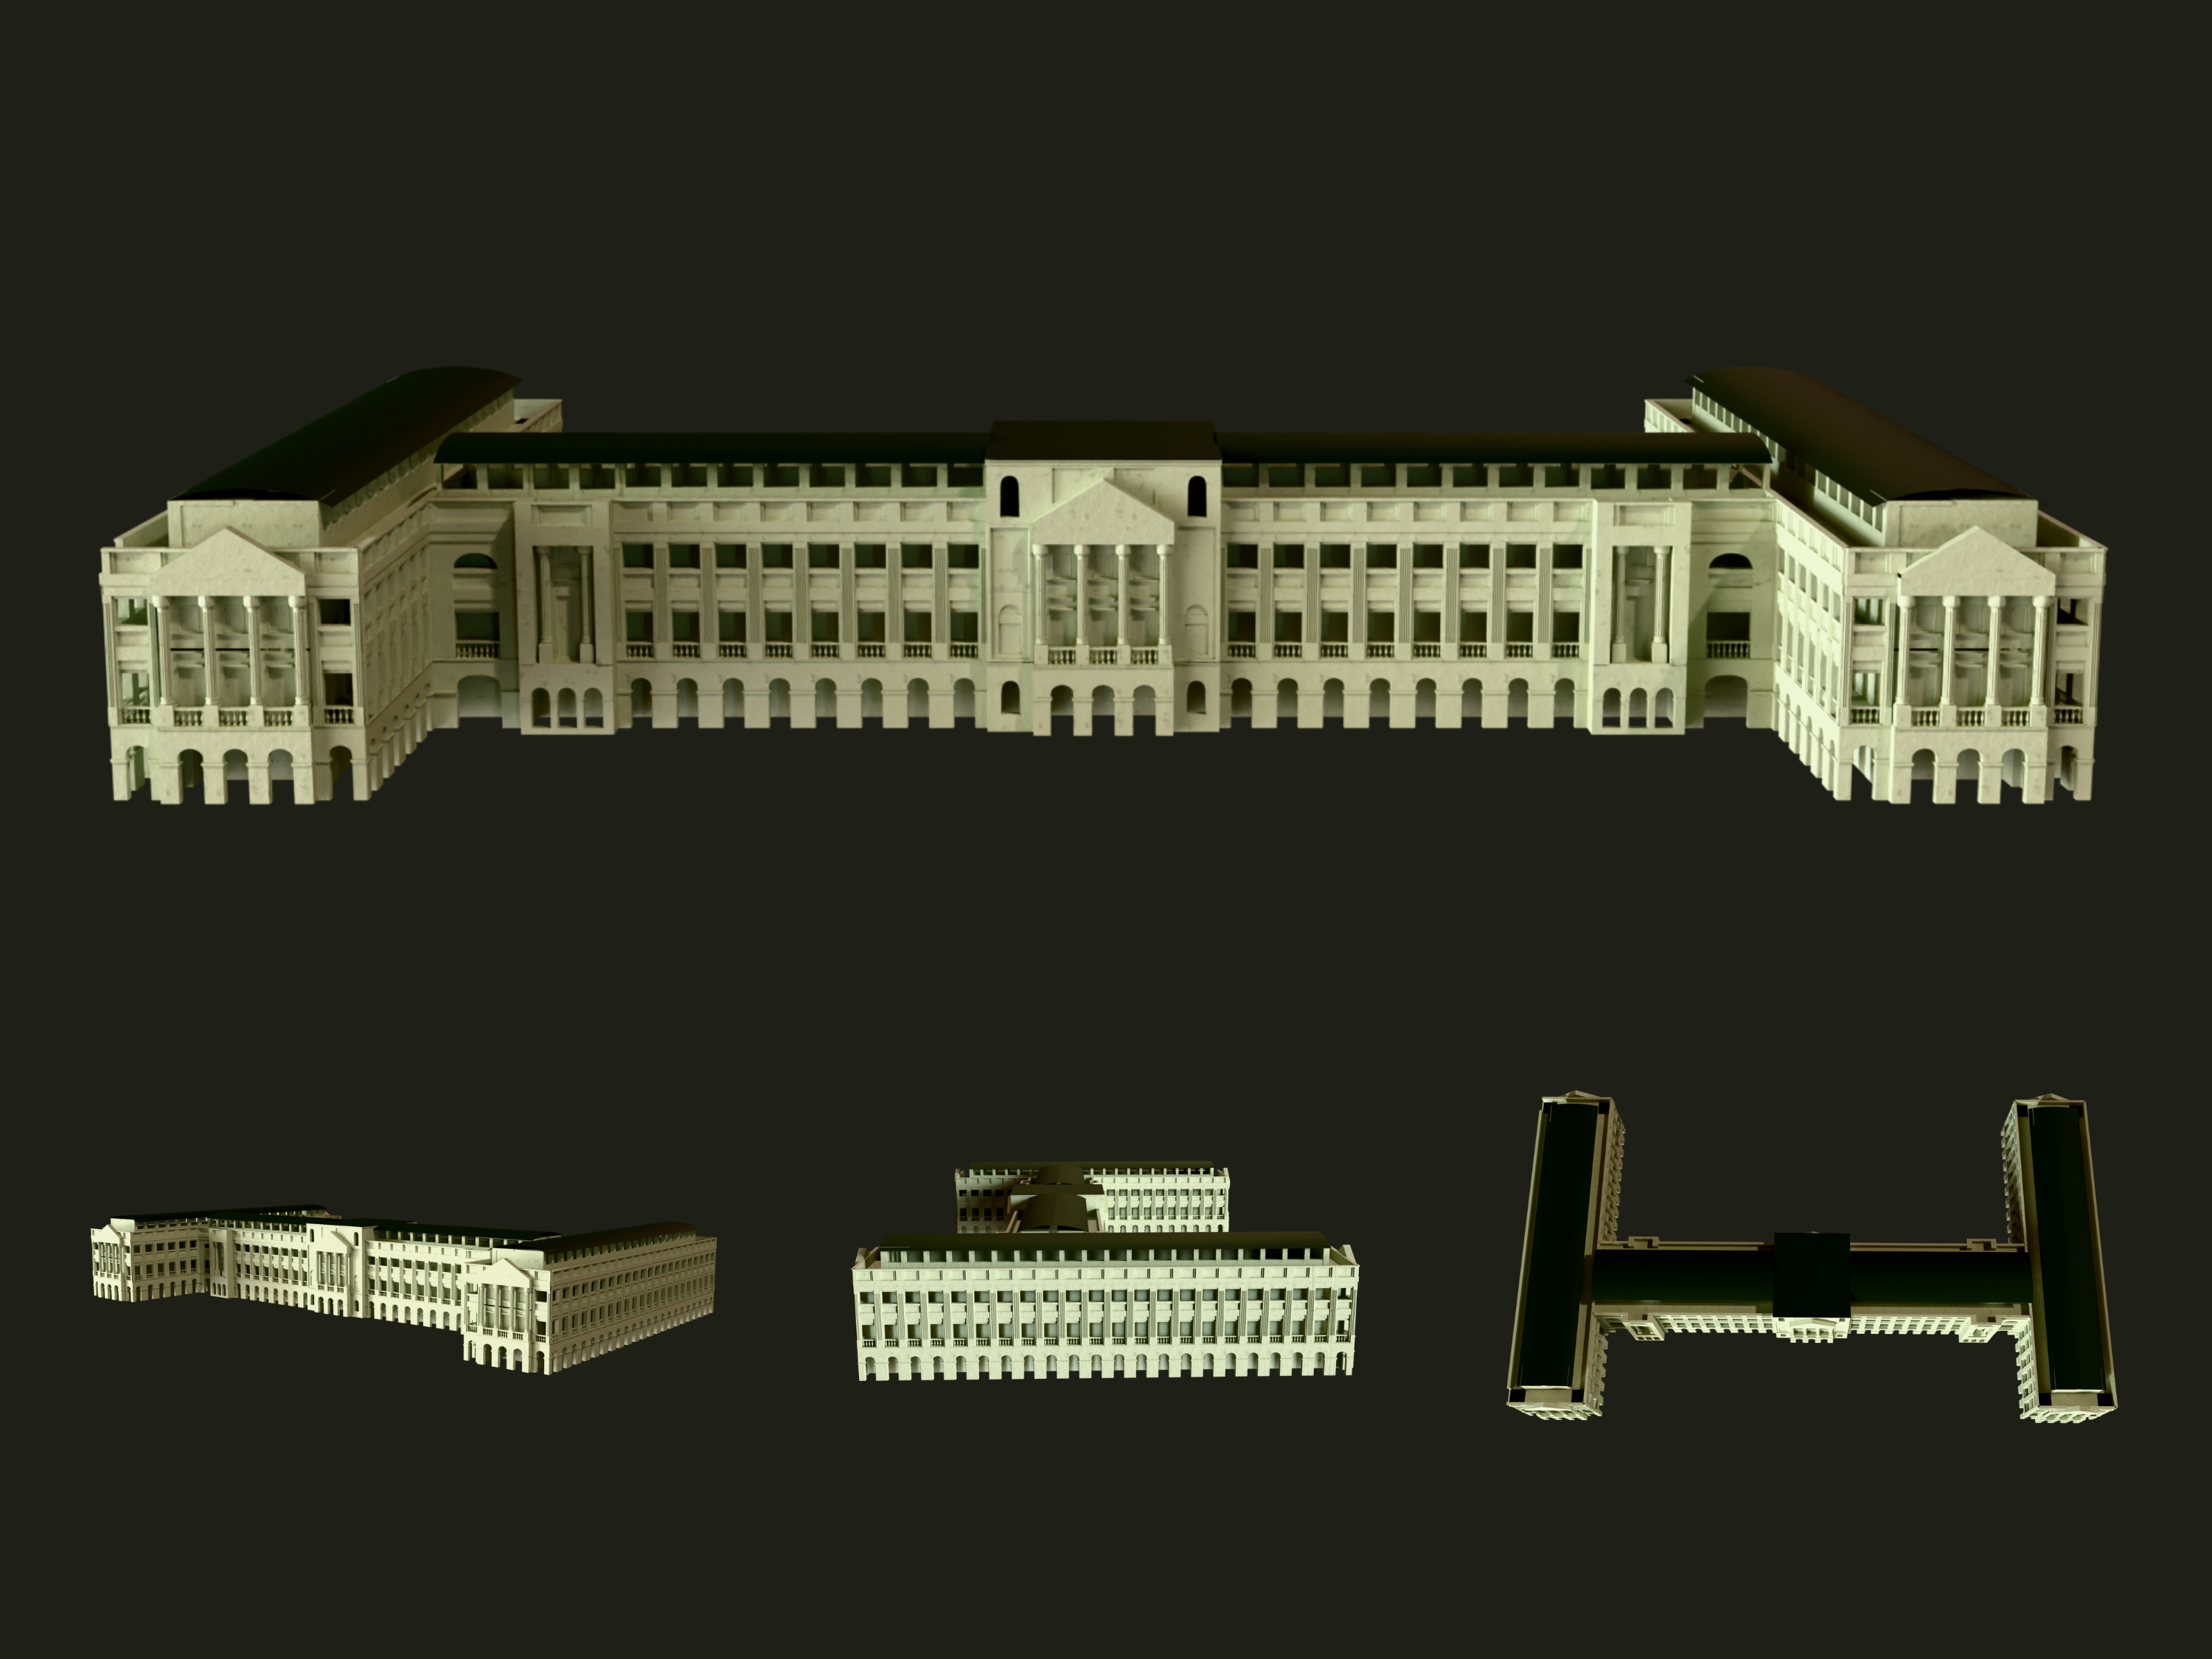
\includegraphics[width=1.0\linewidth]{Intro.png}%
    \caption{Render of the recreated LS Hall in Blender}
    \label{fig:overview_pcg}
\end{figure}

\section{Conclusion}

\subsection{\textbf{3D Asset Collection}}

The project resulted in the creation of a collection of textured 3D modular assets that is easily importable to the specified editor - Anito Builder. This collection of models consists of different types of wall segments that can be duplicated and arranged. It has a complete set of wall segments enough to recreate the overall structure of the LS Hall building in the DLSU Manila campus, with 1 variation for each kind of wall segment and certain limitations for the arrangement of specific ones. However, visual artifacts can be observed which might have resulted from various modelling and texturing mishaps.

\subsection{\textbf{3D Asset development}}

While the model collection is able to recreate the LS Hall, there are still improvements to be made, especially in the modelling process. When arranged to form a structure, the models appear to work and behave appropriately at first glance. However, when observed carefully, artifacts and texturing issues can be seen, specifically on areas where the objects are joined. Reasons for this could be: overlapping meshes, texturing or UV errors, or rendering miscalculations. Since the models are divided into standardized measurements, it is problematic for certain wall segments whenit comes to texturing, specifically the 2-segment and 3-segment models. While most of the 2-segment models do not have any major issues, the 3-segment ones do. The 3-segment model that has four pillars was initially meant to be exported and generated as one whole model. However, due to issues within the editor, it was segmented into several standard segments. Since the models with pillars have subdivision modifiers for clean and detailed curvatures, segmenting them resulted into sharp seams or cuts which are evident in the rendered mages above.

In conclusion, while the models appear to work as intended, a cleaner and more accurate result requires improvements and revisions to the modelling and texturing process. 

\subsection{\textbf{Prototype Evaluation}}

The prototype created is sufficiently equipped to act as a procedural asset generation tool at its current state. It can create environmental assets for games, or pieces of "filler" buildings in games that need much variation between similarly styled buildings. It can be used in city builders, driving simulators, or other types of games wherein the player cannot go into a building's interior.

Further improvements to the prototype include optimizations to the rendering pipeline. As there is observable framerate drops when rendering scenes with large blocks. Furthermore, to improve the viewing experience of users, some rendering features should be implemented. One of which is mipmapping, such that normal textures do not cause a model to appear too noisy when zoomed out. Another is ambient occlusion, such that the edges of geometry are darkened for visual clarity and realism.

\newpage
\bibliographystyle{ACM-Reference-Format}
\bibliography{references}

\begin{thebibliography}{99}

\bibitem{summerville2017}
Summerville, A., Snodgrass, S., Mateas, M., \& Wardrip-Fruin, N. (2017). 
Procedural Content Generation via Machine Learning (PCGML). 
\textit{IEEE Transactions on Games, 10}(3), 257–270.

\bibitem{shaker2016}
Shaker, N., Togelius, J., \& Nelson, M. J. (2016). 
\textit{Procedural Content Generation in Games: A Textbook and an Overview of Current Research}. 
Springer.

\bibitem{lazaridis2024}
Lazaridis, A., \& Fragulis, G. (2024). 
Applications of procedural content generation in modern interactive systems. 
\textit{Journal of Computer Graphics and Virtual Environments}, 12(1), 1–10.

\bibitem{muller2006}
M{\"u}ller, P., Wonka, P., Haegler, S., Ulmer, A., \& Van Gool, L. (2006). 
Procedural modeling of buildings. 
\textit{ACM Transactions on Graphics (TOG)}, 25(3), 614–623.

\bibitem{parish2001}
Parish, Y. I. H., \& M{\"u}ller, P. (2001). 
Procedural modeling of cities. 
\textit{Proceedings of the 28th annual conference on Computer graphics and interactive techniques}, 301–308.

\bibitem{togelius2013}
Togelius, J., Yannakakis, G. N., Stanley, K. O., \& Browne, C. (2013). 
Search-based procedural content generation: A taxonomy and survey. 
\textit{IEEE Transactions on Computational Intelligence and AI in Games}, 3(3), 172–186.

\bibitem{kim2018}
Kim, J., Kim, T., \& Kim, H. (2018). 
Automatic generation of 3D city models using procedural modeling techniques. 
\textit{Automation in Construction}, 87, 1–13.

\bibitem{watson2008}
Watson, B., Müller, P., Wonka, P., Sexton, C., Veryovka, O., \& Fuller, A. (2008). 
Procedural urban modeling in practice. 
\textit{IEEE Computer Graphics and Applications}, 28(3), 18–26.

\bibitem{smith2011}
Smith, G., Whitehead, J., \& Mateas, M. (2011). 
Tanagra: Reactive planning and constraint solving for mixed-initiative level design. 
\textit{IEEE Transactions on Computational Intelligence and AI in Games}, 3(3), 201–215.

\bibitem{togelius2016}
Togelius, J., \& Shaker, N. (2016). 
\textit{Procedural Content Generation for Games}. 
Springer.

\bibitem{summerson1980}
Summerson, J. (1980). 
\textit{The Classical Language of Architecture}. 
Thames and Hudson.

\bibitem{babych2024}
Babych, M. (2024). 
Principles of software modularity and component testing. 
\textit{Software Engineering Journal}, 29(4), 45–56.

\bibitem{ayepeku}
Ayepeku, F. O. (n.d.). 
Low-level programming principles: A guide for developers. 
\textit{Open Source Technical Notes}.

\bibitem{isqtb2014}
International Software Testing Qualifications Board. (2014). 
\textit{Standard Glossary of Terms Used in Software Testing}. 
ISTQB Foundation Level Documentation.

\bibitem{zhang2025}
Zhang, Y. (2025). 
Rule-based generative design in procedural content generation. 
\textit{Proceedings of the IEEE Conference on Games}, 1–6.

\end{thebibliography}

\end{document}
